\chapter{Introduction} \label{chapter:introduction}

\section{Motivation} \label{1:motivation}

    A simple Google search for "getting lost on campus" nets almost 400,000,000 results - hundreds of popular news articles and blog posts telling stories about getting lost on a college campus or giving tips about avoiding such a situation. While Google \cite{albertson2017googlemaps} encourages students to use their product for campus navigation, Google Maps\footnote{\url{https://www.google.com/maps}} as well as similar products (Bing Maps\footnote{\url{https://www.bing.com/maps}}, Apple Maps\footnote{\url{https://www.apple.com/maps/}}) are general-purpose and usually don't meet the needs of students. This property is usually either because they do not have all the updated details about campus buildings or because they do not support indoor navigation for campuses\footnote{\url{https://www.google.com/maps/about/partners/indoormaps/}}.
    
    Universities around the world help their students navigate by providing a printed map. Furthermore, with the rapid advancement of technology, the majority have switched to digital maps, which are often static pictures and do not provide more guidance than a traditional paper map. Some of them have built services on top of Google Maps or similar \acrshort{api}s. However, very few offer much-needed indoor navigation due to its challenges.
    
    % TODO link to SotA
        
    We can therefore identify the need for specialised campus navigation tools and propose an interactive campus map offering indoor and outdoor navigation and additional features.

\section{Environment} \label{1:environment}

    \subsection{University campus} \label{1:university_campus}
        According to a 2007 report \cite{aracis2007raport}
        %TODO: Where to find more recent data?
        by \acrshort{aracis} (\acrlong{aracis}), the campus of \textbf{\acrlong{upb} (\acrshort{upb})} measured around 135.678m\textsuperscript{2} across four different locations in Bucharest, including 68 buildings with 141 lecture halls, 103 seminar rooms and 1025 laboratory rooms.
        
        The university website\footnote{\url{https://upb.ro/}} does not directly provide complete maps of the campus and buildings. However, a virtual tour which includes these maps, as well as 360° panoramas of various campus points of interest (\acrshort{poi}s), has been available\footnote{\url{http://turvirtual.upb.ro/}} since December 2020. Indoor maps of the buildings are not available on the website, allegedly due to concerns that publicly available detailed room information may encourage thievery. However, some unofficial maps made by a university professor are available in the freshmen's guide\footnote{\url{https://www2.slideshare.net/vladposea/ghidul-bobocului-de-la-facultatea-de-automatica-si-calculatoare-vers-20112012}} for the \acrlong{acs}.
        
    \subsection{Faculty application} \label{1:faculty_app}
    
        A group of students at the \acrlong{acs} are currently working on a collaborative application for students which aims to act as an information hub, collecting data that would be relevant for students from different sources \cite{alexandru2020acsupbmobile}. The \gls{opensource} application is available on GitHub\footnote{\url{https://github.com/acs-upb-mobile/acs-upb-mobile}} and includes a timetable (fig. \ref{2:fig:timetable}) where each event has an associated location (classroom, lecture hall etc.). It is based entirely on Google technologies: it uses a cross-platform mobile technology called \gls{flutter}, which allows it to run on Android and iOS devices as well as directly on the web; the database uses Google Cloud, specifically \gls{firebase} cross-platform solutions.
    
        \begin{wrapfigure}[15]{l}{0.52\columnwidth}
            \begin{tabular}{@{}cc@{}}
                \begin{minipage}[b]{0.26\textwidth}
                    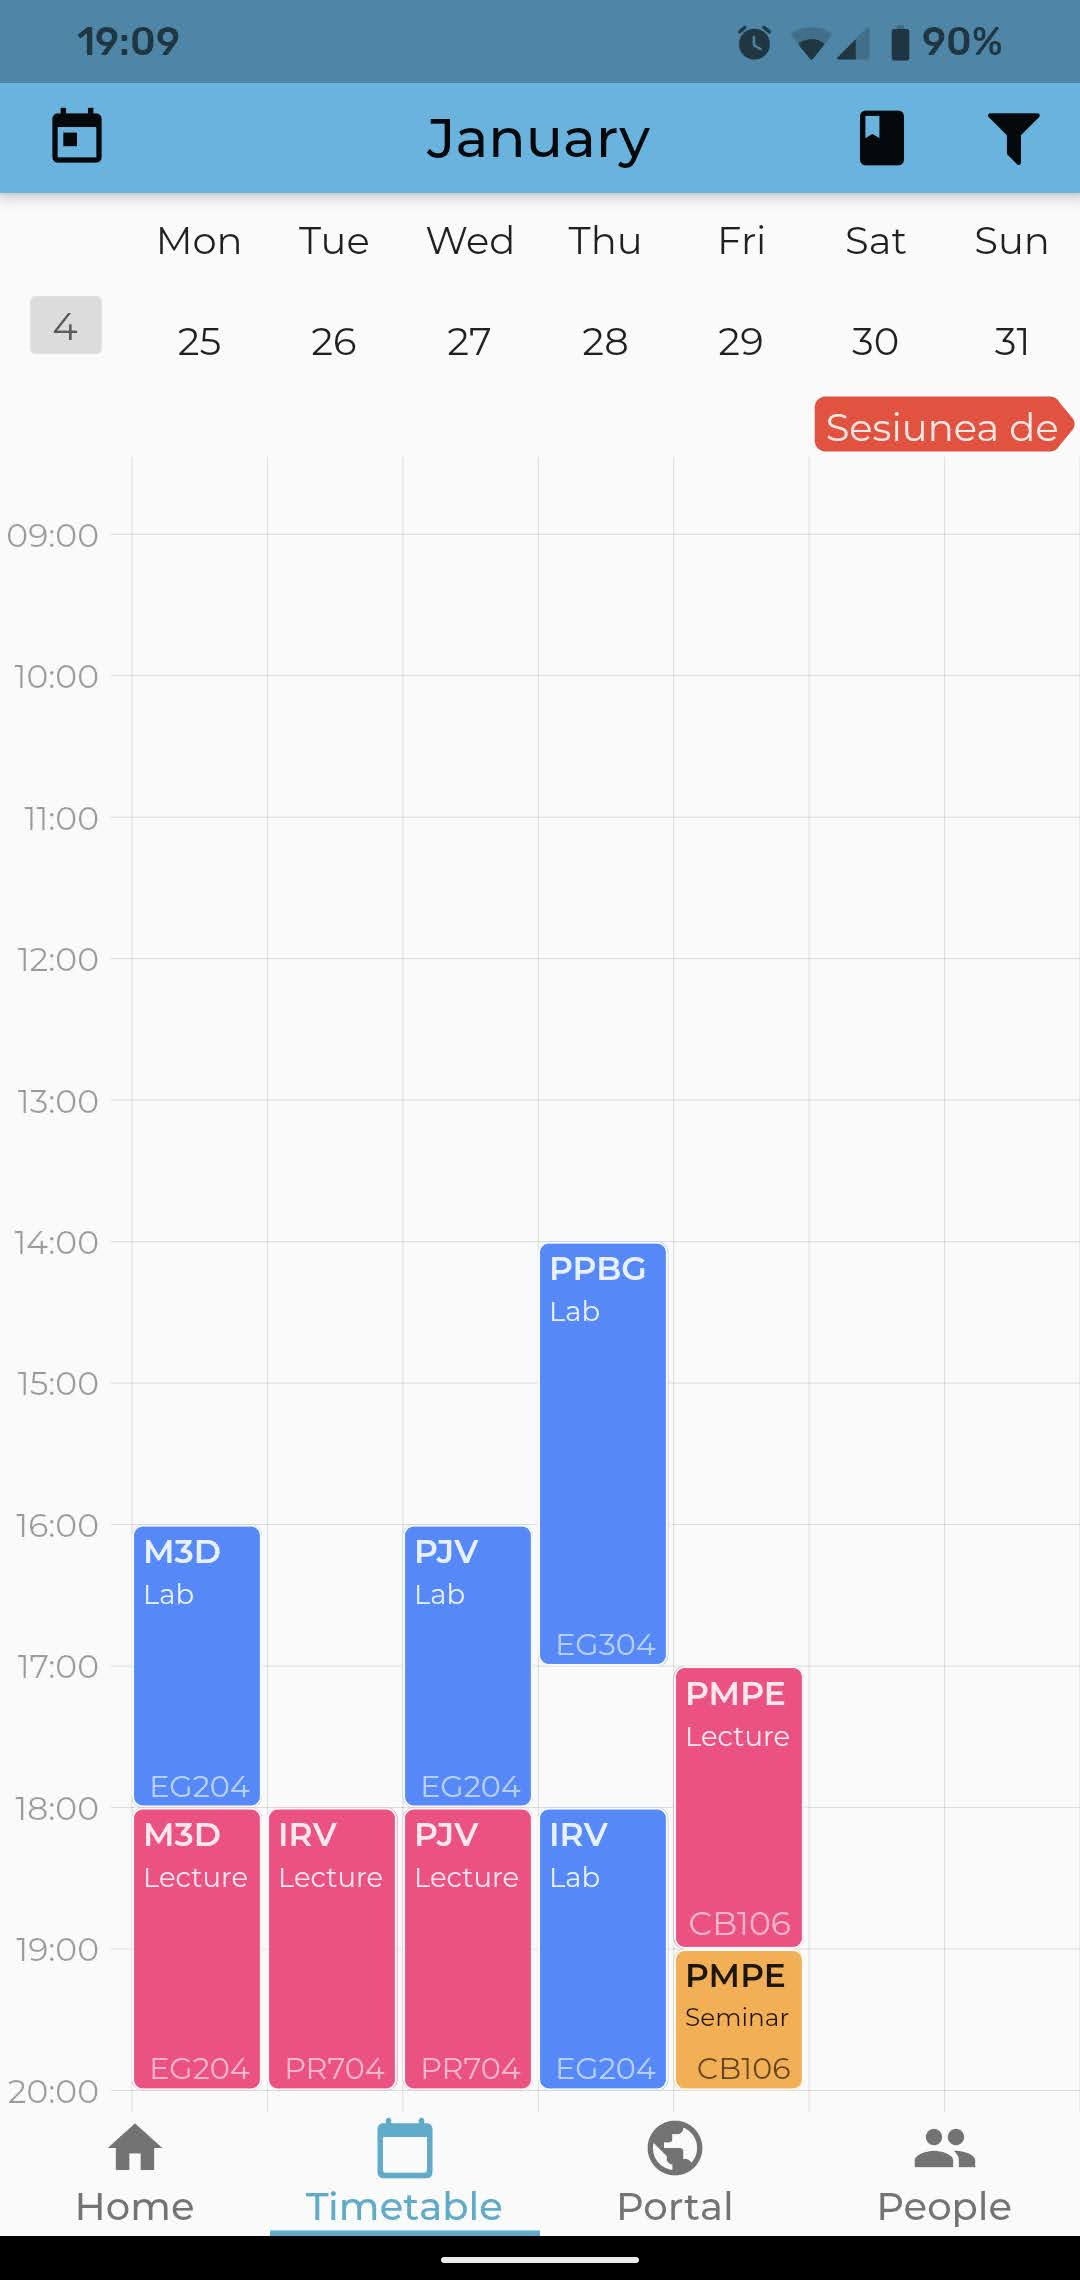
\includegraphics[width=\columnwidth]{figures/app/timetable.jpg}
                    \captionsetup{labelsep=space, textformat=empty}
                    \caption{Screenshot of the Timetable page in the app}   
                    \label{2:fig:timetable}
                \end{minipage}
                \begin{minipage}[b]{0.26\textwidth} 
                    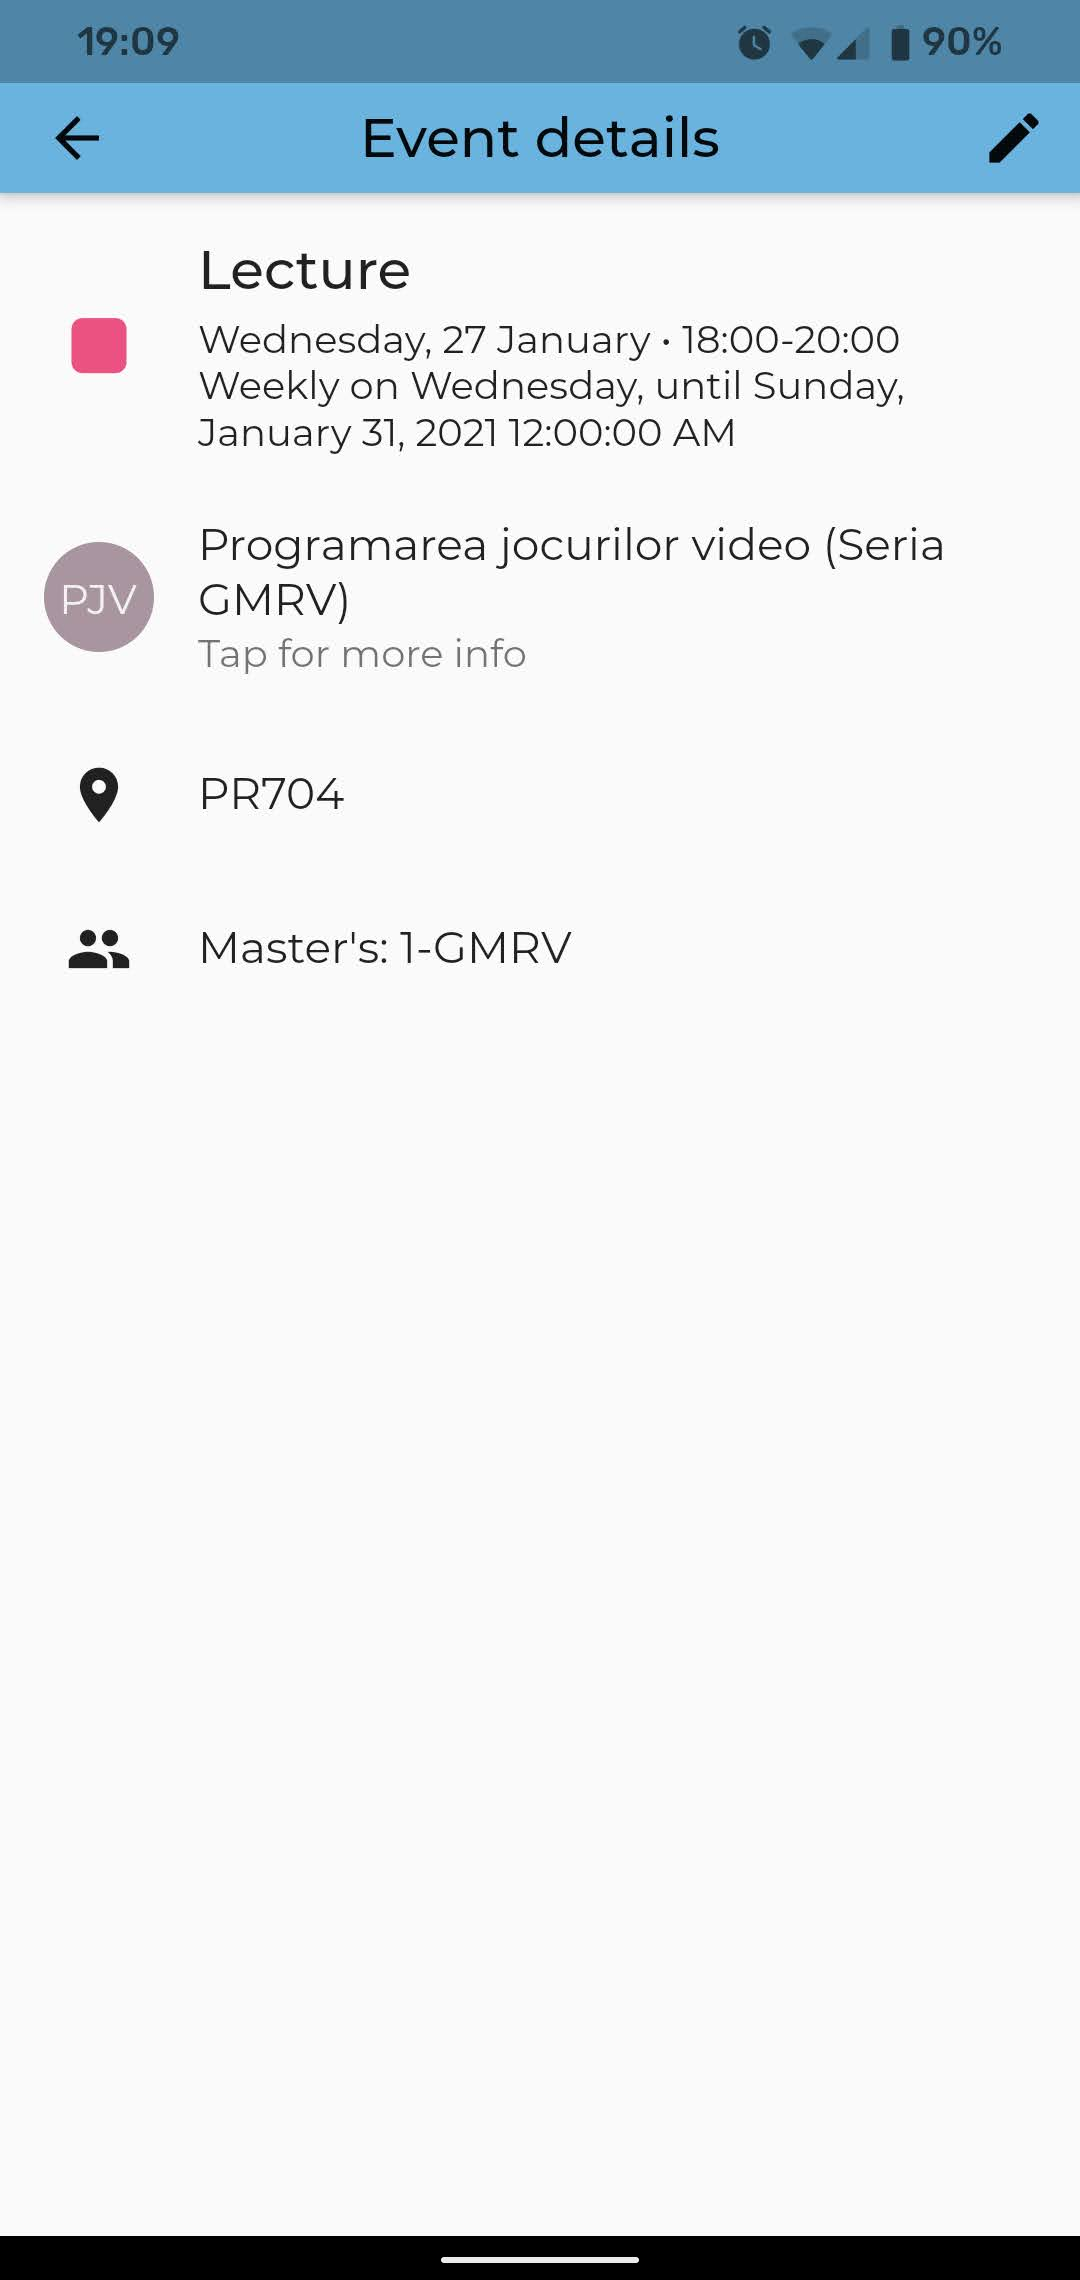
\includegraphics[width=\columnwidth]{figures/app/event.jpg}
                    \captionsetup{labelsep=space, textformat=empty}
                    \caption{Screenshot of the event page in the app}
                    \label{2:fig:event}
                \end{minipage}
            \end{tabular}
        \end{wrapfigure}
        
        Our interactive map aims to be fully compatible with \gls{app}, such that if a user taps on a location in an event page (fig. \ref{2:fig:event}), they would be shown the interactive map as well as navigation instructions to their desired destination.
    
        From here on out in this paper, we will be referring to \gls{app} as \textit{the app}. Additionally, in a similar fashion to the app's paper \cite{alexandru2020acsupbmobile}, we will refer to the larger engineering institution as \textit{the university} or \textit{\acrshort{upb}}, and to the computer science faculty as \textit{the faculty} or \textit{\acrshort{acs}}.
    
\section{Proposed functionalities} \label{1:functionalities}

    As previously stated, the main focus of our tool is to guide students through the university campus. Our proposal as to how navigation should be achieved is described below in section \ref{1:functionalities_core}. However, it is important to note that there is a major caveat associated with any navigation tool that works in a limited area: once the user learns to navigate on their own, the tool's usefulness decreases dramatically. A simple tool that only provides navigation would only be useful in the first few weeks of a semester while the students get used to the classes they need to be in. Subsections \ref{1:functionalities_events} and \ref{1:functionalities_additional} describe additional features that can make the map useful outside of that initial time frame.

    \subsection{Core functionalities} \label{1:functionalities_core}
        At its core, the app needs to be accessible to most or all students, as well as professors and potentially campus visitors. We should not limit ourselves to a single platform, therefore we should aim for the campus navigator to be accessible both on Android as well as iOS devices. Laptops and computers are not targeted, given that it is unlikely that someone would walk around the campus carrying a PC.
    
        In terms of features - first and foremost, the app should provide an \textbf{interactive campus map depicting campus buildings}, and allow the user to zoom/tap on a building to view the \textbf{indoor map per floor} associated with that building. Furthermore, the \textbf{rooms should be labelled} and have an associated type (e.g. classroom, lecture hall, bathroom, office, commercial) that the user can query for. Course and seminar rooms may have additional information, such as the number of seats. Moreover, \textbf{other relevant \acrshort{poi}s} such as coffee or food machines should also be displayed. Additionally, the user should be able to view the 360° view of an area from the \textbf{virtual tour}\footnote{\url{http://turvirtual.upb.ro/}}, where available. Finally, the user should be able to \textbf{save their favourite locations} as well as \textbf{select the types of markers} they wish to see on the map (e.g. hide virtual tour markers, show only bathrooms etc.).
        
        While outdoor navigation can be easily achieved through a service such as Google Maps Platform\footnote{\url{https://developers.google.com/maps}}, indoor navigation is difficult to achieve without specialised hardware (such as Bluetooth beacons) due to attenuation caused by construction rendering GPS unusable indoors. Since innovation in the field of indoor positioning is outside the scope of this project, the initial version of this tool (\textit{v0}) aims to provide \textbf{navigation \textit{without} accurate localisation}. This functionality can be achieved by allowing the user to select their starting position (listing possible options based on approximate location) and their destination. Upon starting navigation, the user can then manually mark a navigation step as complete to see the following step.
        
    \subsection{Events support} \label{1:functionalities_events}
    
        Section \ref{1:faculty_app} describes the application that we wish our map to work with. One-way interaction is rather straightforward: the user presses a location name in the timetable, which queries that location in the map tool and shows a result. Similar interaction can be achieved with external apps and services as well, through intents\footnote{\url{https://developer.android.com/training/basics/intents/filters}} (on Android) and URL Schemes\footnote{\url{https://developer.apple.com/documentation/xcode/allowing_apps_and_websites_to_link_to_your_content/defining_a_custom_url_scheme_for_your_app}} (on iOS). For example, an external website or application (even a Facebook event) can display a campus location name and, if the user presses the name, open our application with the corresponding location query. Students could also use this functionality to share meeting points between them.
        
        Two-way interaction is also possible - in the case of \gls{app} - and could significantly improve the usefulness of our map. If the map has access to timetable and event information from the app, it can display things like events happening nearby, increasing event visibility. For example, suppose a user presses on a classroom. In that case, they could see which class is currently happening there, according to the timetable\footnote{\url{http://acs.pub.ro/~cpop/orare_sem2/Orar_sali_laborator_calculatoare2019_2020sem2.xls}}. Furthermore, a feature that would be particularly useful for event organisers, professors and teaching assistants would be the ability to see which class is available at a specific point in time (ideally including room size/available seating).
        
    \subsection{Additional functionalities} \label{1:functionalities_additional}
    
        Attaching even more information to a location could also be helpful. For instance, a user can add a comment to a location mentioning that it is temporarily closed. Similarly, coffee and food machines could have a rating attached (users can rate them based on the quality of the product) and a label that shows whether they are out of order. Sharing documents/files/announcements in a location could also be done through integration with a project that is still under development called AirDocs. AirDocs is a middleware system that allows placing and retrieving objects or documents at different indoor locations without requiring a positioning system (see appendix \ref{a:airdocs} for more information).
        
        Following Waze\footnote{\url{https://www.waze.com/}}'s example, we could also add gamification elements to our map, such as achievements for locations visited and distance travelled. Furthermore, in a similar fashion to Google Maps monthly reports, we can show statistics such as campus location where the user has spent the most time in. Furthermore, the app could support organising events such as treasure hunts/scavenger hunts on campus grounds.

\section{Outline} \label{1:outline}
    \textbf{Chapter \ref{chapter:sota}} outlines the current state of the art, in terms of existing technologies, services and applications related to our project.
    
    \textbf{Chapter \ref{chapter:implementations}} compares several different implementation approaches for the navigation problem.
    
    \textbf{Chapter \ref{chapter:user_study}} looks at the student's opinions on the topic of campus navigation needs through the lens of our user study.
    
    \textbf{Chapter \ref{chapter:conclusion}} offers an overview of the learnings from our study, and discusses potential next steps.